Karo pabėgėliu mėnesinis skaičius pagal šalis\cite{refugees} buvo sutrauktas į bendrą per mėnesinį pasaulio babėgėlių skaičių 2003 - 2017 metais.
Žodžio „war“ skaičius per mėnesį buvo surinktas iš ABC naujienų portalo antraščių\cite{abcNews} tuo pačiu laikotarpiu.

\begin{figure}
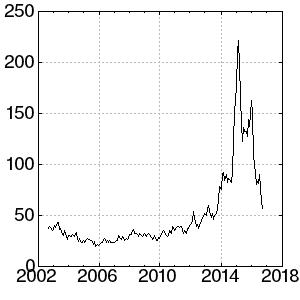
\includegraphics[scale=0.65]{../scripts/refugees_war/refugees.png}
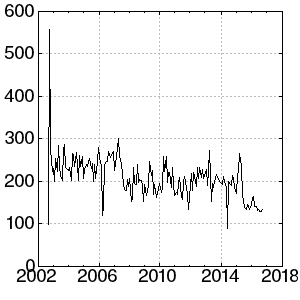
\includegraphics[scale=0.65]{../scripts/refugees_war/war.png}
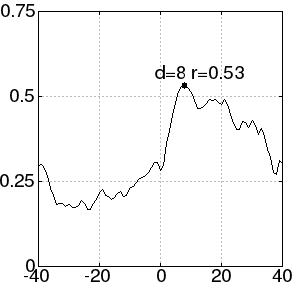
\includegraphics[scale=0.65]{../scripts/refugees_war/result.png}
    \caption{Grafikas kairėje: vidutinis mėnesinis karo pabėgėlių skaičius pasaulyje (tūkstančiais). Grafikas centre: mėnesinis „war“ skaičius ABC naujienų antraštėse. Grafikas dešinėje: signalų tarpusavio koreliacija}
\end{figure}

Nors tarp karo pabėgėlių ar žodžio „war“ dažnumo grafiko akivaizdaus ryšio nesimato,
poros koreliacijos funkcija rodo didžiausią signalų panašumą \( R_{fg}(t) = 0.53 \), kai \( t = 8 \).
Signalų porą galima klasifikuoti kaip vidutiniškai koreliuojančia tarpusavyje.
Koreliacijos grafikas parodo, kad didžiausias pabėgėlių skaičius fiksuojamas praėjus vidutiniškai aštuoniems mėnesiams po didžiausio žiniasklaidos susidomėjimo.
Žodžio „war“ dumenys gali būti klaidinantys ir iškreipiantys tikrąją koreliaciją, nes neįvertina klaidingų sutapimų (false positives), kaip dažnai naudojamas angliškas posakis „war on drugs“ ir pan.
Taip pat,rezultatus būtų galima patikslinti, atrinkus antraštes su „war“ ir šalies pavadinimu, ir patikrinus koreliaciją su pabėgėlių skaičiumi iš tos šalies.
